\section{Subreddits}

How subreddits change over time (by cohort)

One way to look at reddit is as a multi-community social network. Each subreddit can be considered as a semi-independent community, and as such, we can study the evolution of these communities based on time, cohorts and survivability.  A number of other online communities have similar properties, with tighter (Wikiprojects, enterprise social network discussion groups) or looser (Wikia, StackOverflow) interdependence between the individual sub-communities.

One of the initial question we can ask is how is the number of posts in these surviving communities evolving? One thing to be aware here though is that this variable is likely to be sensitive to the ration of active users per active subreddits. If we imagine that users don't change their posting patterns rapidly, and increased number of users per subreddits implies in an increased number of posts per subreddit. The overall number of users per subreddits, however, seems fairly stable throughout the years.

Figure N shows the evolution of number of posts per active subreddits in time for subreddits created between 2008 and 2013. We can observe that the average number of posts per subreddit increases over time. Since the ratio of active users per subreddit remains relatively stable, one could imagine that subreddits are receiving more posts throughout the time.

\begin{figure}[!tb]
\centering
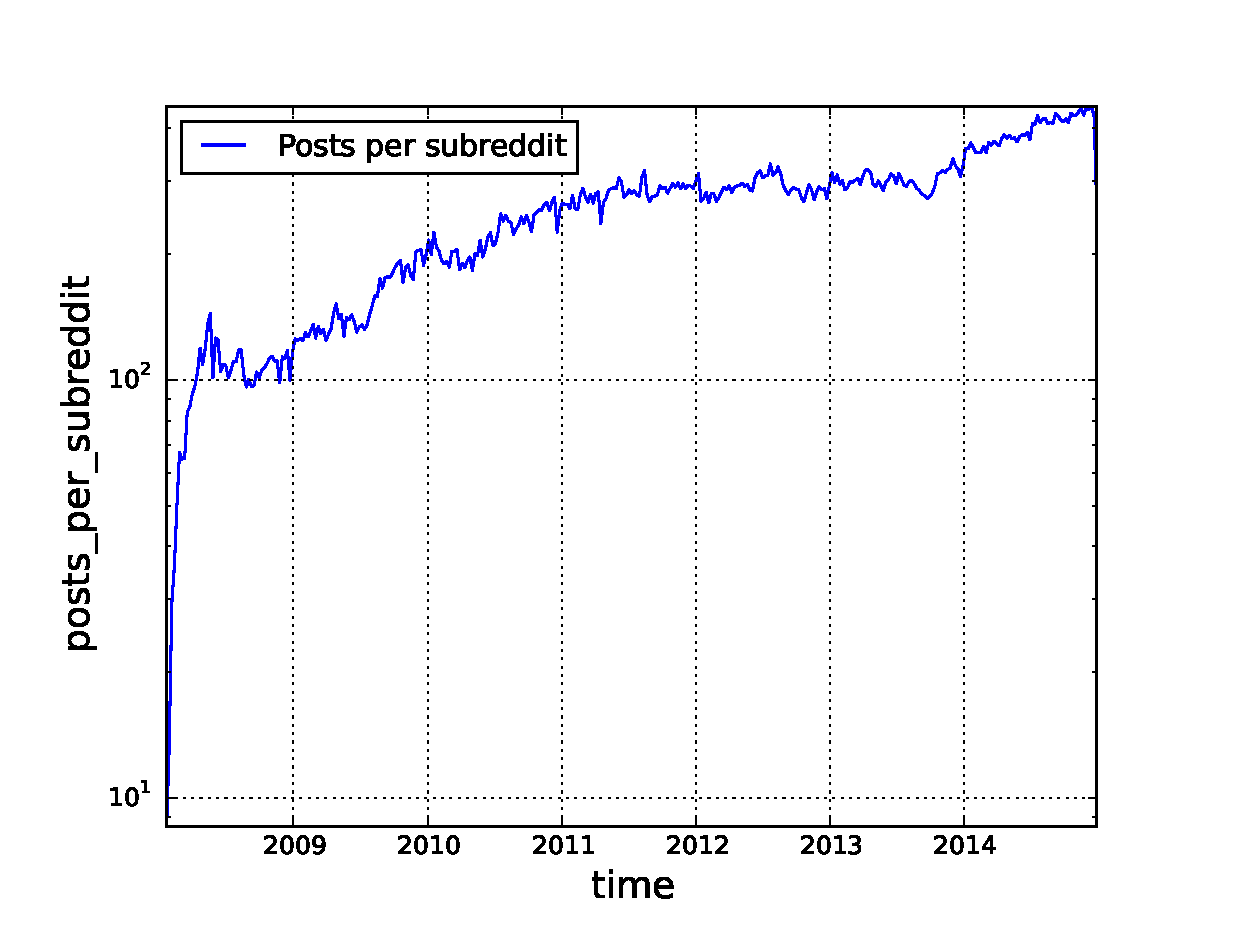
\includegraphics[scale=0.4]{./images/posts_per_subreddit_over_time_total.eps}
\caption{Caption}
\label{fig:posts_per_subreddit_over_time_total}
\end{figure}

To better understand how correct is this conclusion, we cohort the subreddits in time. We can observe that the majority of posts in reddit are made in 2008 subreddits, and the posting averages for this cohort dominates the total posting average for the whole social network. Also, we notice that for most points in time, the number of posts per subreddits increases as we move to older cohorts. This, however, is not sufficient for us to conclude that these communities are evolving in different ways, since subreddits from older cohorts had more time to consolidate their reach and popularity and most of the ``likely to die'' subreddits that bring the average number of posts down in newer cohorts are still alive.

\begin{figure}[!tb]
\centering
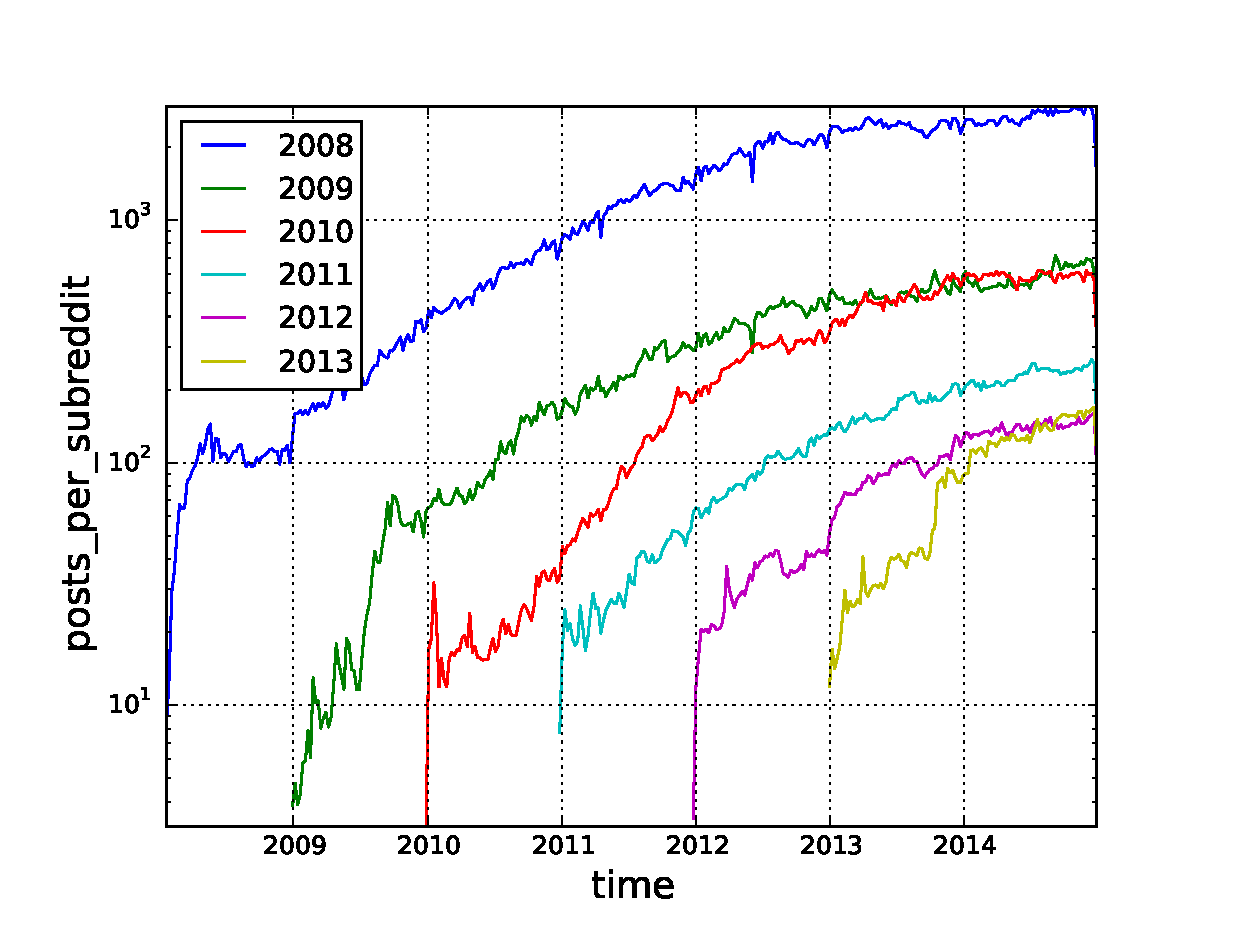
\includegraphics[scale=0.4]{./images/posts_per_subreddit_over_time_cohorts.eps}
\caption{Caption}
\label{fig:posts_per_subreddit_over_time_cohorts}
\end{figure}

To properly compare these communities starting from the same baseline, we evaluate every posting time according to the subreddit creation time (fists post ever made in the subreddit). The x-axis then becomes the time the subreddit has lived, grouped by cohort. This approach reveals a general trend of subreddits from newer cohorts stabilizing in a lower posting average than older cohorts. This, however, does not hold true for the 2009 and 2010 cohorts, although they stabilize in very similar levels, and for the 2013 cohort, for which we have only one year of data in the overlap for all subreddits.

\begin{figure}[!tb]
\centering
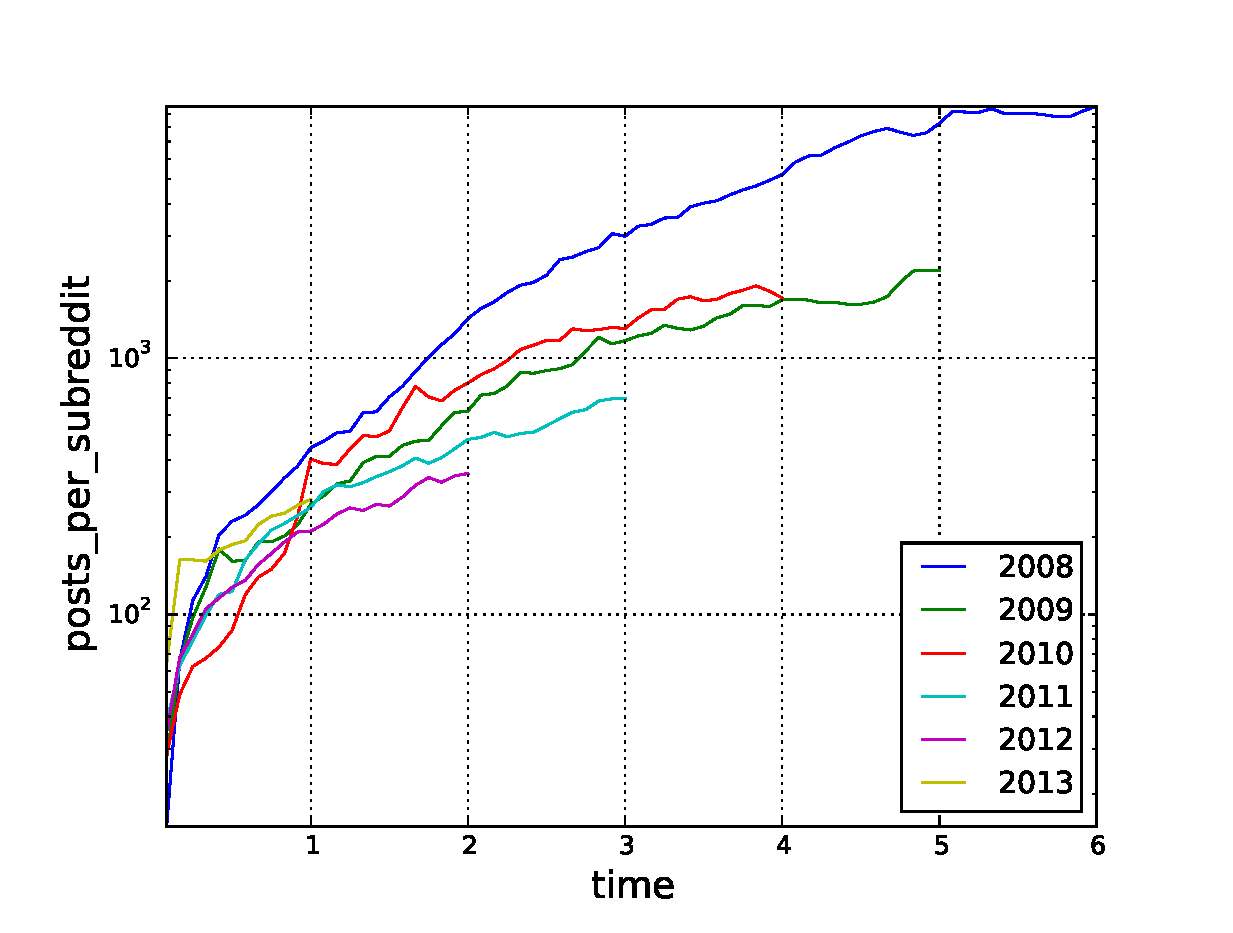
\includegraphics[scale=0.4]{./images/posts_per_subreddit_cohorts.eps}
\caption{Caption}
\label{fig:posts_per_subreddit_cohorts}
\end{figure}

Assuming that subreddits that survive have, on average, a higher number of posts than the ones that do not survive, part of the higher levels of posting for the older cohorts could also be explained by a faster ``death rate'' of the low posting subreddits. Therefore, the faster the number of posts per subreddit grows, the faster the non-fit subreddits are being eliminated.

Subreddit Survival

Similarly to what we did for users, we look in a one year time window for the last post that was created for each subreddit and define as subreddits that died as the ones that the last post happened in the first nine months of the one year window. The Kaplan-Meier curve is shown in Figure N.

\begin{figure}[!tb]
\centering
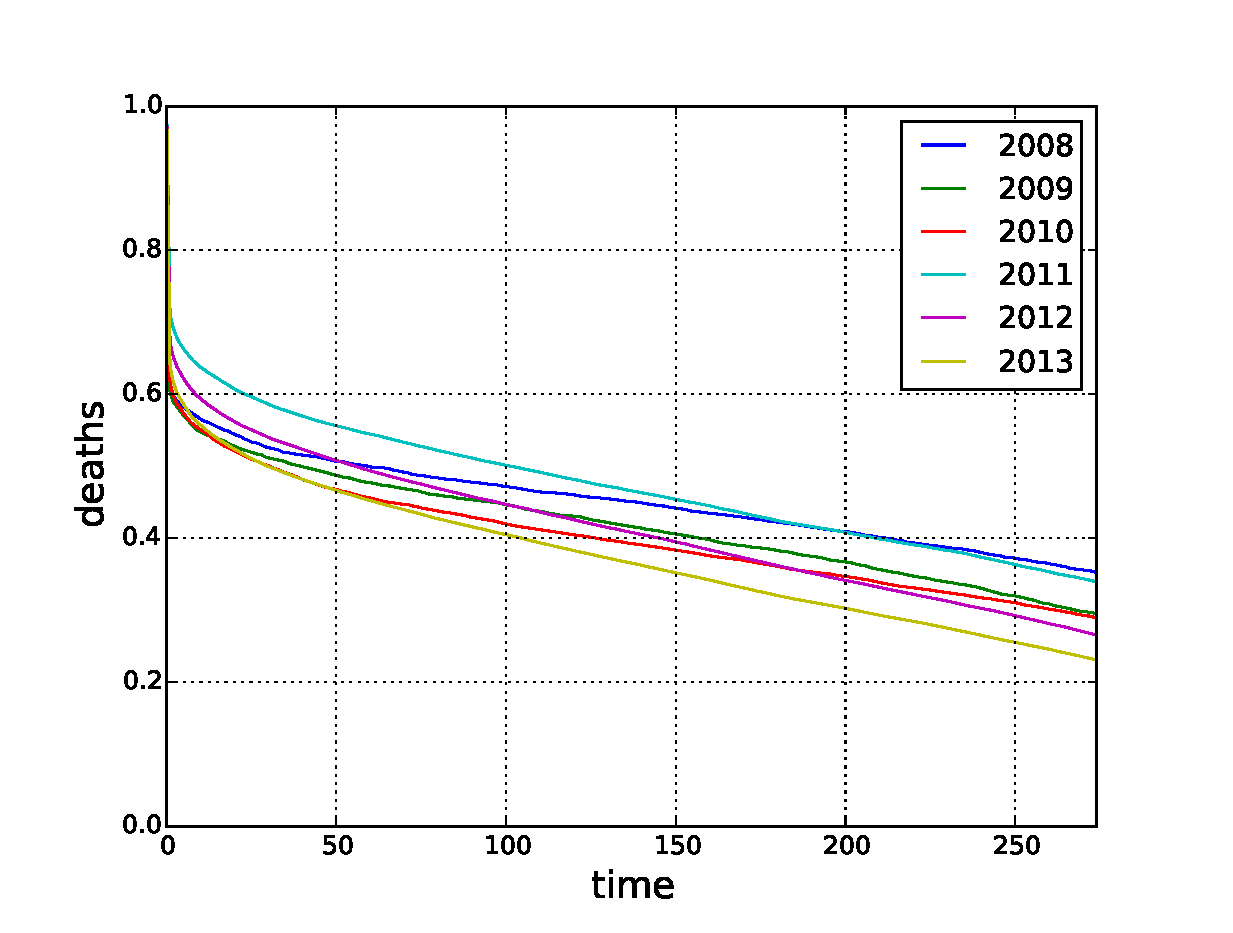
\includegraphics[scale=0.4]{./images/kaplan_meier_subreddits.eps}
\caption{Caption}
\label{fig:kaplan_meier_subreddits}
\end{figure}

In this survival curve, we also observe that there is a significant number of subreddits that survive only through the first day, just as seen with the users, although the proportion in this case is not as high as the users . Also, unlike the users, there are significantly differences in the ``decay of subreddits''.
